\label{chap:communication}
\label{sec:communication}

This chapter describes the communication interface between the GUI and the Userspace. The central part of the interface are Remote Procedure Calls, described in XXX, YYY and ZZZ, but some of the sequences span more than one RPC: these are further described in XXX.

\section{Remote Procedure Calls}
% (Ruda)

We use GWT RPCs.

TODO: describe GWT RPCs

They are asynchronous, always called from the client. They return an instance of the return type on success or an instance of an exception on failure.

\section{Communication Scheme}
GUI communicates with Userspace via a GWT RemoteService implementation, defined as the FilmTitService interface.
The interface provides asynchronous RPC methods (the responses are processed by callbacks).

The method is always called from the client, because Javascript security policies do not allow to handle incoming calls.
Therefore, in case the Userspace needs to actively contact the GUI without the GUI having sent a request before,
this has to be implemented in the GUI by polling.

\section{Manipulating Documents}
\subsection{Whole Document Operations}

\subsubsection{DocumentResponse createNewDocument(String sessionID, String documentTitle, String movieTitle, String language, String moviePath)}

Creates the document
(without source chunks, which have to be added by calling saveSourceChunks),
returns its id, together with media source suggestions based on movieTitle.
     	
\subsubsection{Void selectSource(String sessionID, long documentID, MediaSource selectedMediaSource)}
Sets the media source of the document.

\subsubsection{List<Document> getListOfDocuments(String sessionID)}
Returns all documents owned by the user, ordered by date and time of last change.

\subsubsection{Document loadDocument(String sessionID, long documentID)}
Returns the document with the given id, with source chunks but without translation suggestions.

\subsubsection{Void closeDocument(String sessionID, long documentId)}
Not used. TODO: delete?
     	
\subsubsection{Void changeDocumentTitle(String sessionId, long documentID, String newTitle)}
Sets a different title for the document.
     	
\subsubsection{List<MediaSource> changeMovieTitle(String sessionId, long documentID, String newMovieTitle)}
Returns media source suggestions based on newMovieTitle.
The movie title is not changed yet,
this is only done on calling selectSource.
TODO: is this true?     	 
     	
\subsubsection{Void deleteDocument(String sessionID, long documentID)}
Remove the given document from the list of user's documents.
(The data might not be discarded immediately
as the translations still might be used to enc�ich the translation memory)	 

\subsection{Source Subtitles Operations}

\subsubsection{Void saveSourceChunks(String sessionID, List<TimedChunk> chunks)}
Save the given source chunks as the contents of the given document
(which was already created by calling createNewDocument)	 

\subsubsection{Void setChunkStartTime(String sessionID, ChunkIndex chunkIndex, long documentId, String newStartTime)}
Change the start time of the given chunk to the new value.

\subsubsection{Void setChunkEndTime(String sessionID, ChunkIndex chunkIndex, long documentId, String newEndTime)}
Change the end time of the given chunk to the new value.

\subsubsection{Void setChunkTimes(String sessionID, ChunkIndex chunkIndex, long documentId, String newStartTime, String newEndTime)}
Change the start time and end time of the given chunk to the values.

\subsubsection{TranslationResult changeText(String sessionID, TimedChunk chunk, String newDbForm)}
Change the source text of the chunk,
resulting in new translation suggestions
which are sent as the result.

\subsubsection{Void deleteChunk(String sessionID, ChunkIndex chunkIndex, long documentId)}
Remove the chunk from the document, together with its translation if it exists.

\subsection{Target Subtitles Operations}

\subsubsection{TranslationResult getTranslationResults(String sessionID, TimedChunk chunk)}
Get the list of possible translations of the given chunk.

Userspace passes the given chunk to the core, which generates zero or more translation suggestions.
These are packed into a TranslationResult instance and sent back to GUI.

\subsubsection{List<TranslationResult> getTranslationResults(String sessionID, List<TimedChunk> chunks)}
Get the list of lists of possible translations of the given chunks.

\subsubsection{Void stopTranslationResults(String sessionID, List<TimedChunk> chunks)}
Stop generating translation results for the given chunks
(to be used when the getTranslationResults call has been called
with the given chunks.

\subsubsection{Void setUserTranslation(String sessionID, ChunkIndex chunkIndex, long documentId, String userTranslation, long chosenTranslationPairID)}
Set the user translation of the given chunk.

This method is called once the user selects a suggested translation and optionally post-edits it
(or does not select one but inputs the translation text directly).
The translation is then saved by Userspace;
the id of the TranslationPair chosen for post-editing is also sent, providing feedback which then can be used to improve future suggestions.

\section{User Registration and Login}

The user is required to log in to be able to save his work on the server.

The user is logged in if he has a valid session id which is linked to a user account in Userspace.
The session id expires after a given period of time without any user interaction with the server,
it is therefore neccessary that the user can log in without the application\'s main window being reloaded so that the user does not lose unsaved data.

Two ways to log in -- Simple Login and OpenID. Only Logout is common, other methods devided into two subsections.


\subsubsection{Void logout(String sessionID)}
Invalidate the user session with the given sessionID


\subsection{Simple Login and Registration}
\label{subsec:simple_login}

TODO: There is simple login which is very simple. See Figure \ref{gui:sd:simple_login}.

TODO: probably split the diagram into two (or delete the logout completely from the diagram, there is nothing interesting on it)

\begin{figure}[h]
\begin{center}
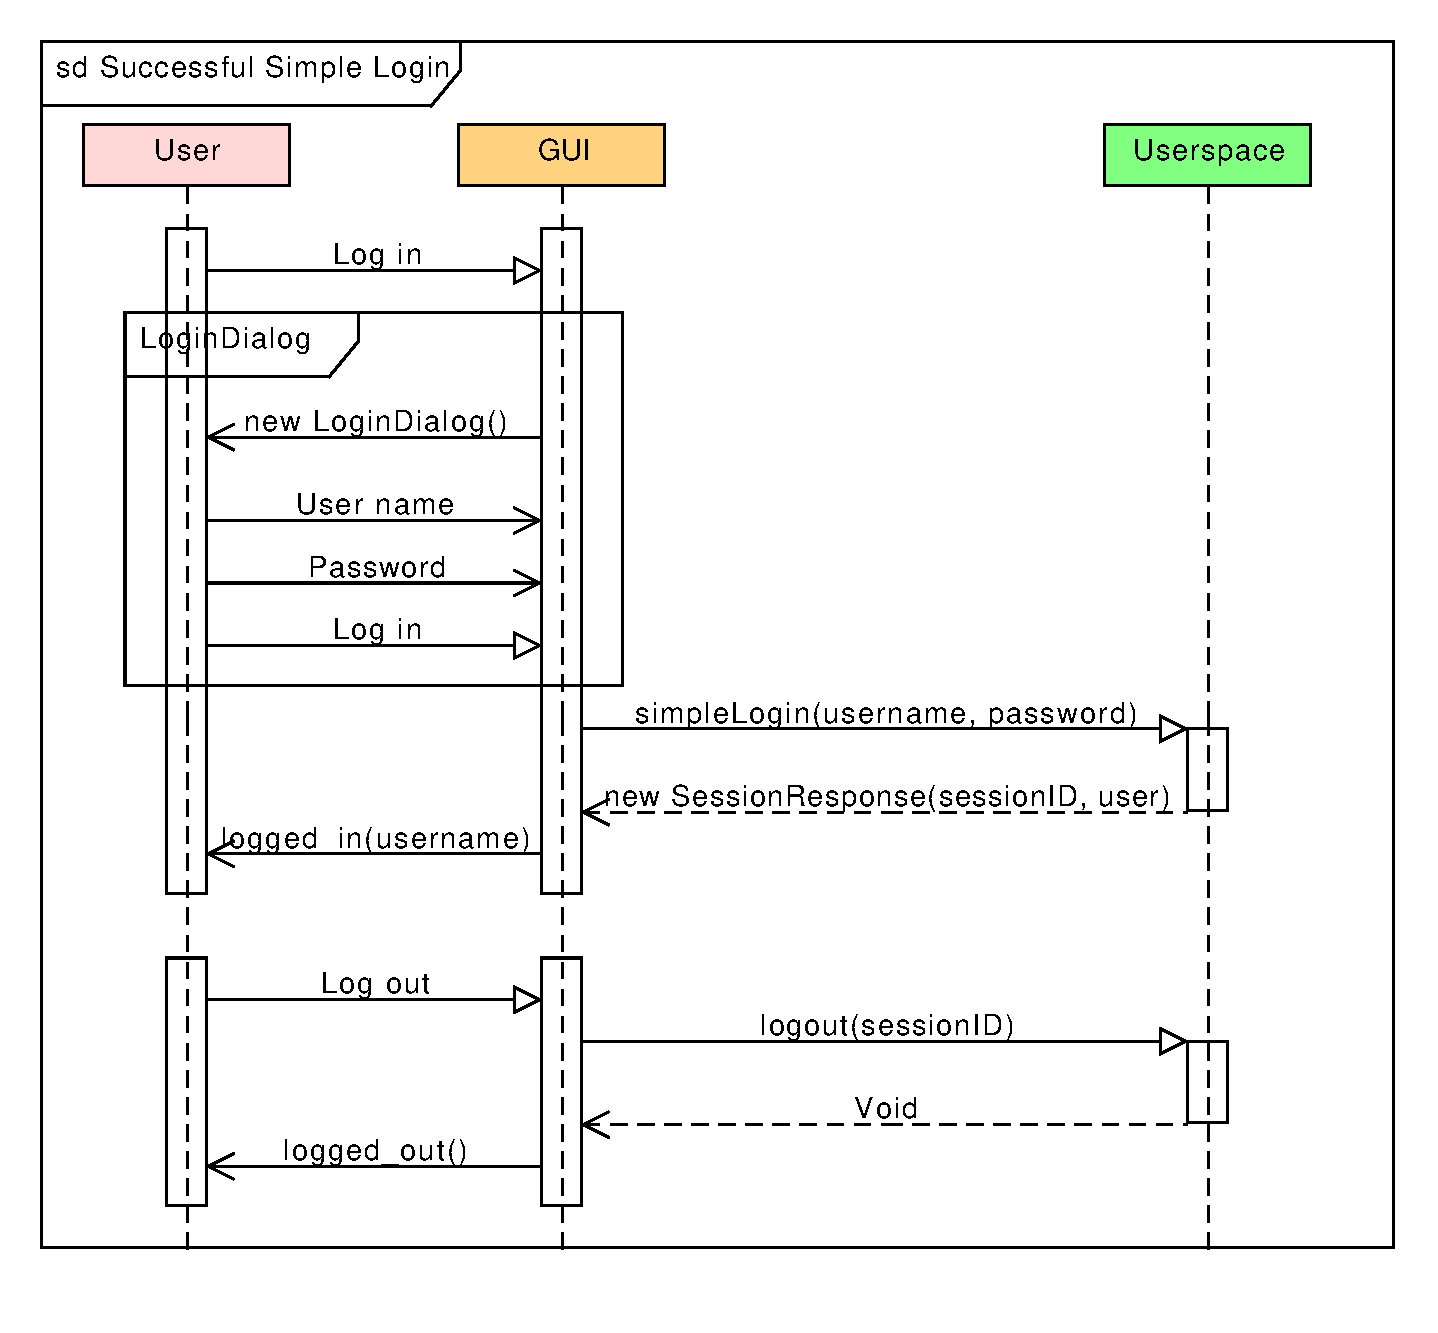
\includegraphics[scale=0.65]{figures/simple_login_sequence.pdf}
\end{center}
\caption{Sequence diagram of simple login and logout.}\label{gui:sd:simple_login}
\end{figure}

\subsubsection{Boolean registration(String username, String password, String email, String openId)}
Register a user with the given username and password, setting the given e-mail and sending registration info to it.
@return true if successful, false if not
TODO: throw an exception


\subsubsection{SessionResponse simpleLogin(String username, String password);}
Try to log in the user with the given username and password.
@return SessionResponse containing the sessionID and the User object on success, null on error
TODO: throw an exception


\subsubsection{SessionResponse checkSessionID(String sessionID);}
Validates the given sessionID.
@param sessionID
@return SessionResponse containing the sessionID and the User object if the sessionID is valid, null if not


\subsubsection{Boolean sendChangePasswordMail(String username);}
Send an email with a link to password reset
to the user's email address.
@param username registered username of the user
@return true on success, false if username is incorrect or there is no email address
TODO: throw an exception


\subsubsection{Boolean sendChangePasswordMailByMail(String email)}
Send an email with a link to password reset
to the user's email address.
@param email registered e-mail address of the user
@return true on success, false if username is incorrect or there is no email address
TODO: throw an exception

    

\subsubsection{Boolean changePassword(String username, String password, String token);}
Change password in case of forgotten password;
user chooses a new password,
user authentication is done by the token sent to user's email
@return true on success, false if token is invalid
TODO: throw an exception

\subsection{Login via OpenID Services}
\label{subsubsec:gui_openid}

No registration needed, user automatically registered on first login.

TODO: move partly to last section (Complex Operations) and maybe partly to GUI

The authentication itself is done in a new authentication window.
A successful authentication is then paired with the GUI instance using a temporary one-time identifier, authID, shared by the main window and the authentication window.
(Because of Javascript security restrictions, there is no simple way of sending the result of the authentication process from the authentication window to the main window;
however, it is straightforward to generate the authID in the main window, store it in Userspace and send it to the authentication window on its creation.)

When the main window requests user authentication, it generates the authID, calls getAuthenticationURL and opens an authentication window with the returned URL.
Then it waits for the user to authenticate in the authentication window
-- the waiting is active, polling the Userspace with getSessionID in regular intervals.
TODO: I suggest every 3 seconds for the first 2 minutes, then every 10 seconds for the following 8 minutes, and then every 30 seconds forever.
And, of course, if the main window regains focus, we call getSessionID immediately.
For each of the authentication services, there is a webpage that enables the user to authenticate
(its URL is returned by getAuthenticationURL)
and then passes information about the result of the authentication to a webpage given to it as a get parameter
(we use the Authentication Response Window as the target webpage).
The result is then sent to Userspace by validateAuthentication.
If the authentication is successful, a new session is created for the user.
The main window then acquires the new session id via getSessionID and the authentication process is completed.

Currently supported OpenID providers are Google, Yahoo and Seznam.

\subsubsection{LoginSessionResponse getAuthenticationURL(AuthenticationServiceType serviceType);}
Get the URL of a window to show to the user for him to log in using his OpenID

Called by GUI when authentication is required and the user is not logged in (i.e. does not have a valid sesion id).
A temporary one-time identifier, authID, is generated for the authentification session only to identify the client logging in and sent to Userspace together with the request.
The chosen service to be used for authentication is also given (e.g. Google or Facebook).
The Userspace returns a URL of the webpage to be used for authentication.

\subsubsection{Boolean validateAuthentication(int authID, String responseURL);}
Send the URL of the response from the OpenID provider to Userspace for validation.

Called from the authentication response window after the user\'s attempt to authenticate themself.
The responseURL contains information from the authentication service to be checked and used by the Userspace.
If the authentication is found to have been successful, a new session is generated for the user and paired with the given authID, and true is returned.
Otherwise, the method returns false.

\subsubsection{SessionResponse getSessionID(int authID)}
Poll the Userspace to find out whether the user has already successfully logged in using his OpenID.

Userspace checks whether a successful authentication has been done with the given authID.
If yes, the corresponding session id is returned.
Otherwise, null is returned.
TODO null or empty string?
TODO we still need to be able to send info that the user decided to cancel the authentication if we find this out - probably by an exception?

\section{User Settings}

There are several settings that the user can change. There is a separate call for each of the settings -- therefore, a set of indivdual calls must be invoked if the user decides to change multiple settings at once, and each of the calls can succeed or fail independently on the results of the other calls.

The settings are stored in the User object and sent to GUI on login, as a part of the SessionResponse which is the result of the methods simpleLogin, getSessionID and checkSessionID. There is no dedicated method to load the settings; checkSessionID is to be used for that purpose.

\subsection{Account and Logging in Settings}

\subsubsection{Void setUsername(String sessionID, String username)}
Change user's username.

\subsubsection{Void setPassword(String sessionID, String password)}
Change user's password.

\subsubsection{Void setEmail(String sessionID, String email)}
Change user's e-mail.

\subsubsection{Void setPermanentlyLoggedIn(String sessionID, boolean permanentlyLoggedIn)}
Stay logged in permanently (for 1 month) instead of 1 hour (sets the session timeout)

\subsection{Translation Workspace Settings}

\subsubsection{Void setMaximumNumberOfSuggestions(String sessionID, int number)}
Set maximum number of suggestions to show for each line.

\subsubsection{Void setUseMoses(String sessionID, boolean useMoses)}
Include MT results in translation suggestions.

\section{Remote logging}
    

\subsubsection{Void logGuiMessage(LevelLogEnum level, String context, String message, String sessionID);}
Log the given message from GUI on server.

\section{Exceptions Thrown by RPCs}

The RPCs typically throw an exception on failure. These exceptions should be of only four types, described in this section.

\subsection{InvalidSessionIdException}

Most of the RPCs can only be invoked by a logged in user -- such RPCs take the sessionID as a parameter and throw an InvalidSessionIdException in case of an invalid sessionID. Typically the ID would be originally valid but expired, so the expected reaction to this exception is to simply ask the user to log in again.

\subsection{InvalidDocumentIdException}

RPCs that manipulate the document usually take the documentID as a parameter and throw an InvalidDocumentIdException if a document with the given ID does not exist or does not belong to the user.

\subsection{InvalidChunkIdException}

RPCs that manipulate individual chunks take either the whole chunks or only their indexes as a parameter. They throw an InvalidChunkIdException if the specified chunk does not exist.

\subsection{InvalidValueException}

The InvalidValueException is thrown by a method if a value provided by the user, such as an e-mail address or a password, does not have the required format. It always contains details about the nature of the error as the message, which usually should be shown to the user.

\section{Complex Operations}

In most cases, one RPC is sufficient to perform the whole operation. However, sometimes a whole sequence of several RPCs is required to complete one complex operation. Such operations are described in this section.

\subsection{Document Creation}

\begin{figure}[h]
\begin{center}
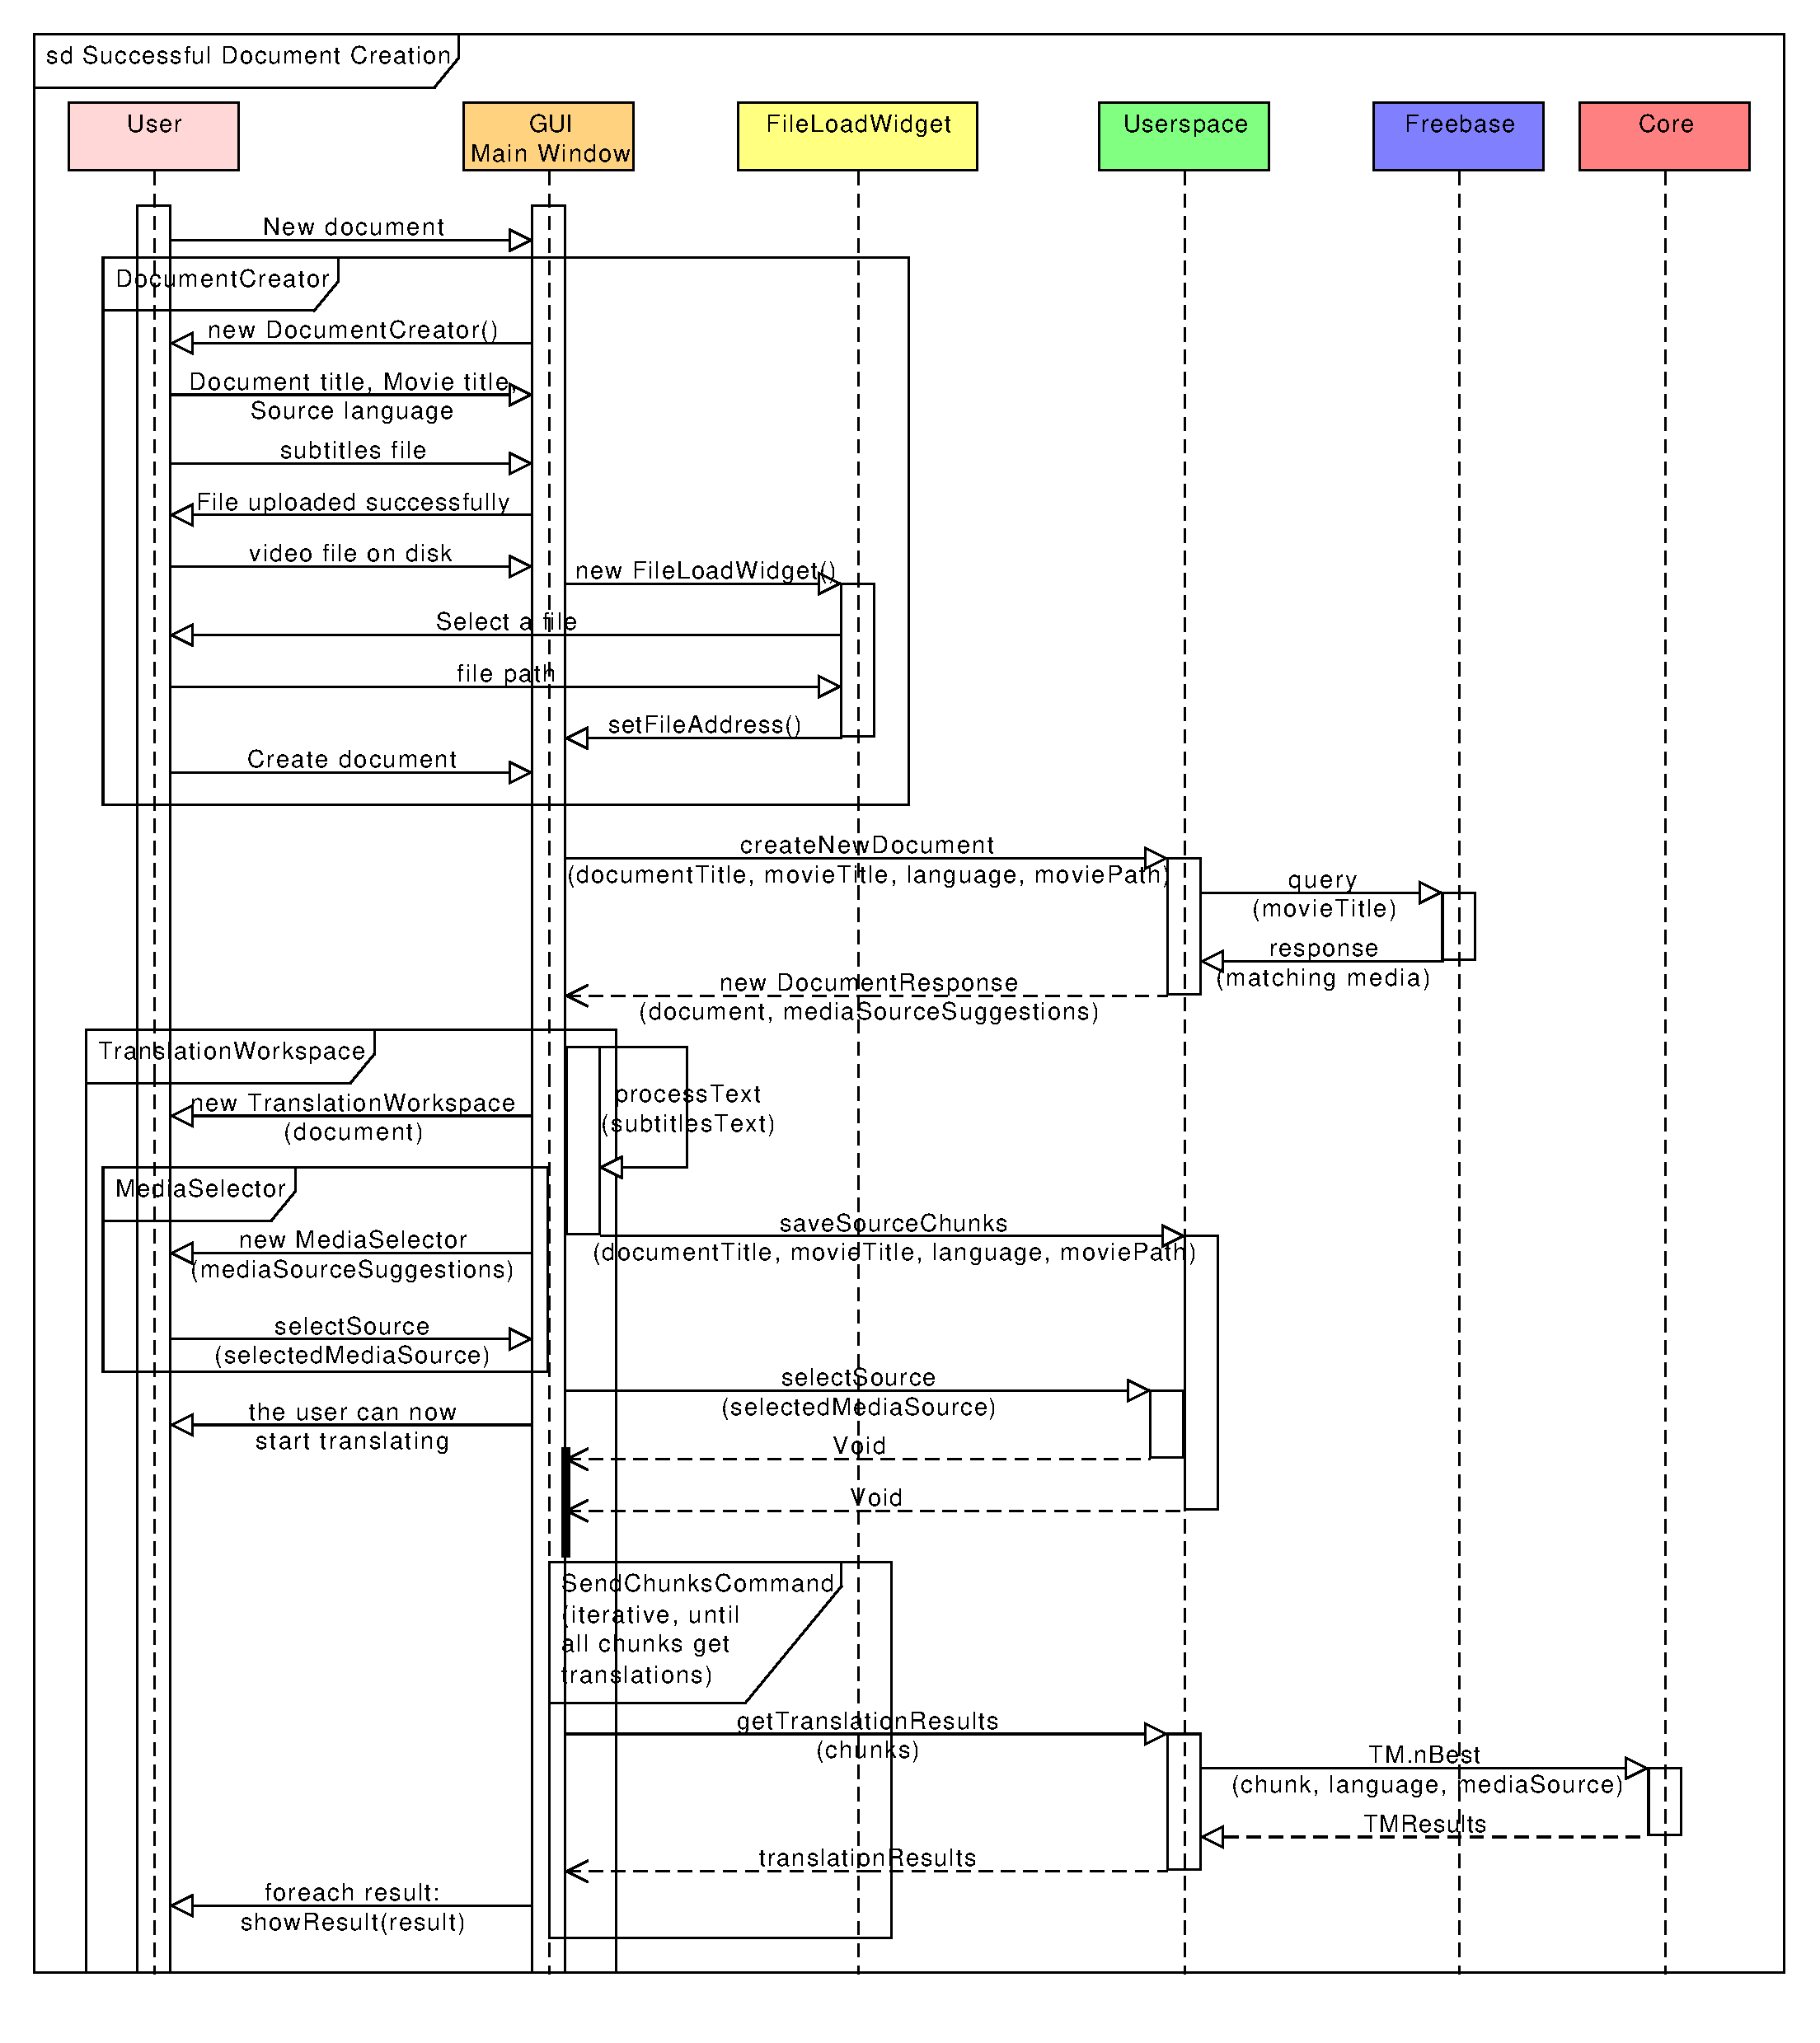
\includegraphics[scale=0.45]{figures/document_creation_sequence.pdf}
\end{center}
\caption{Sequence diagram of document creation, including translation suggestions loading.}\label{gui:sd:document_creation}
\end{figure}

\subsection{OpenID Login}

\begin{figure}[h]
\begin{center}
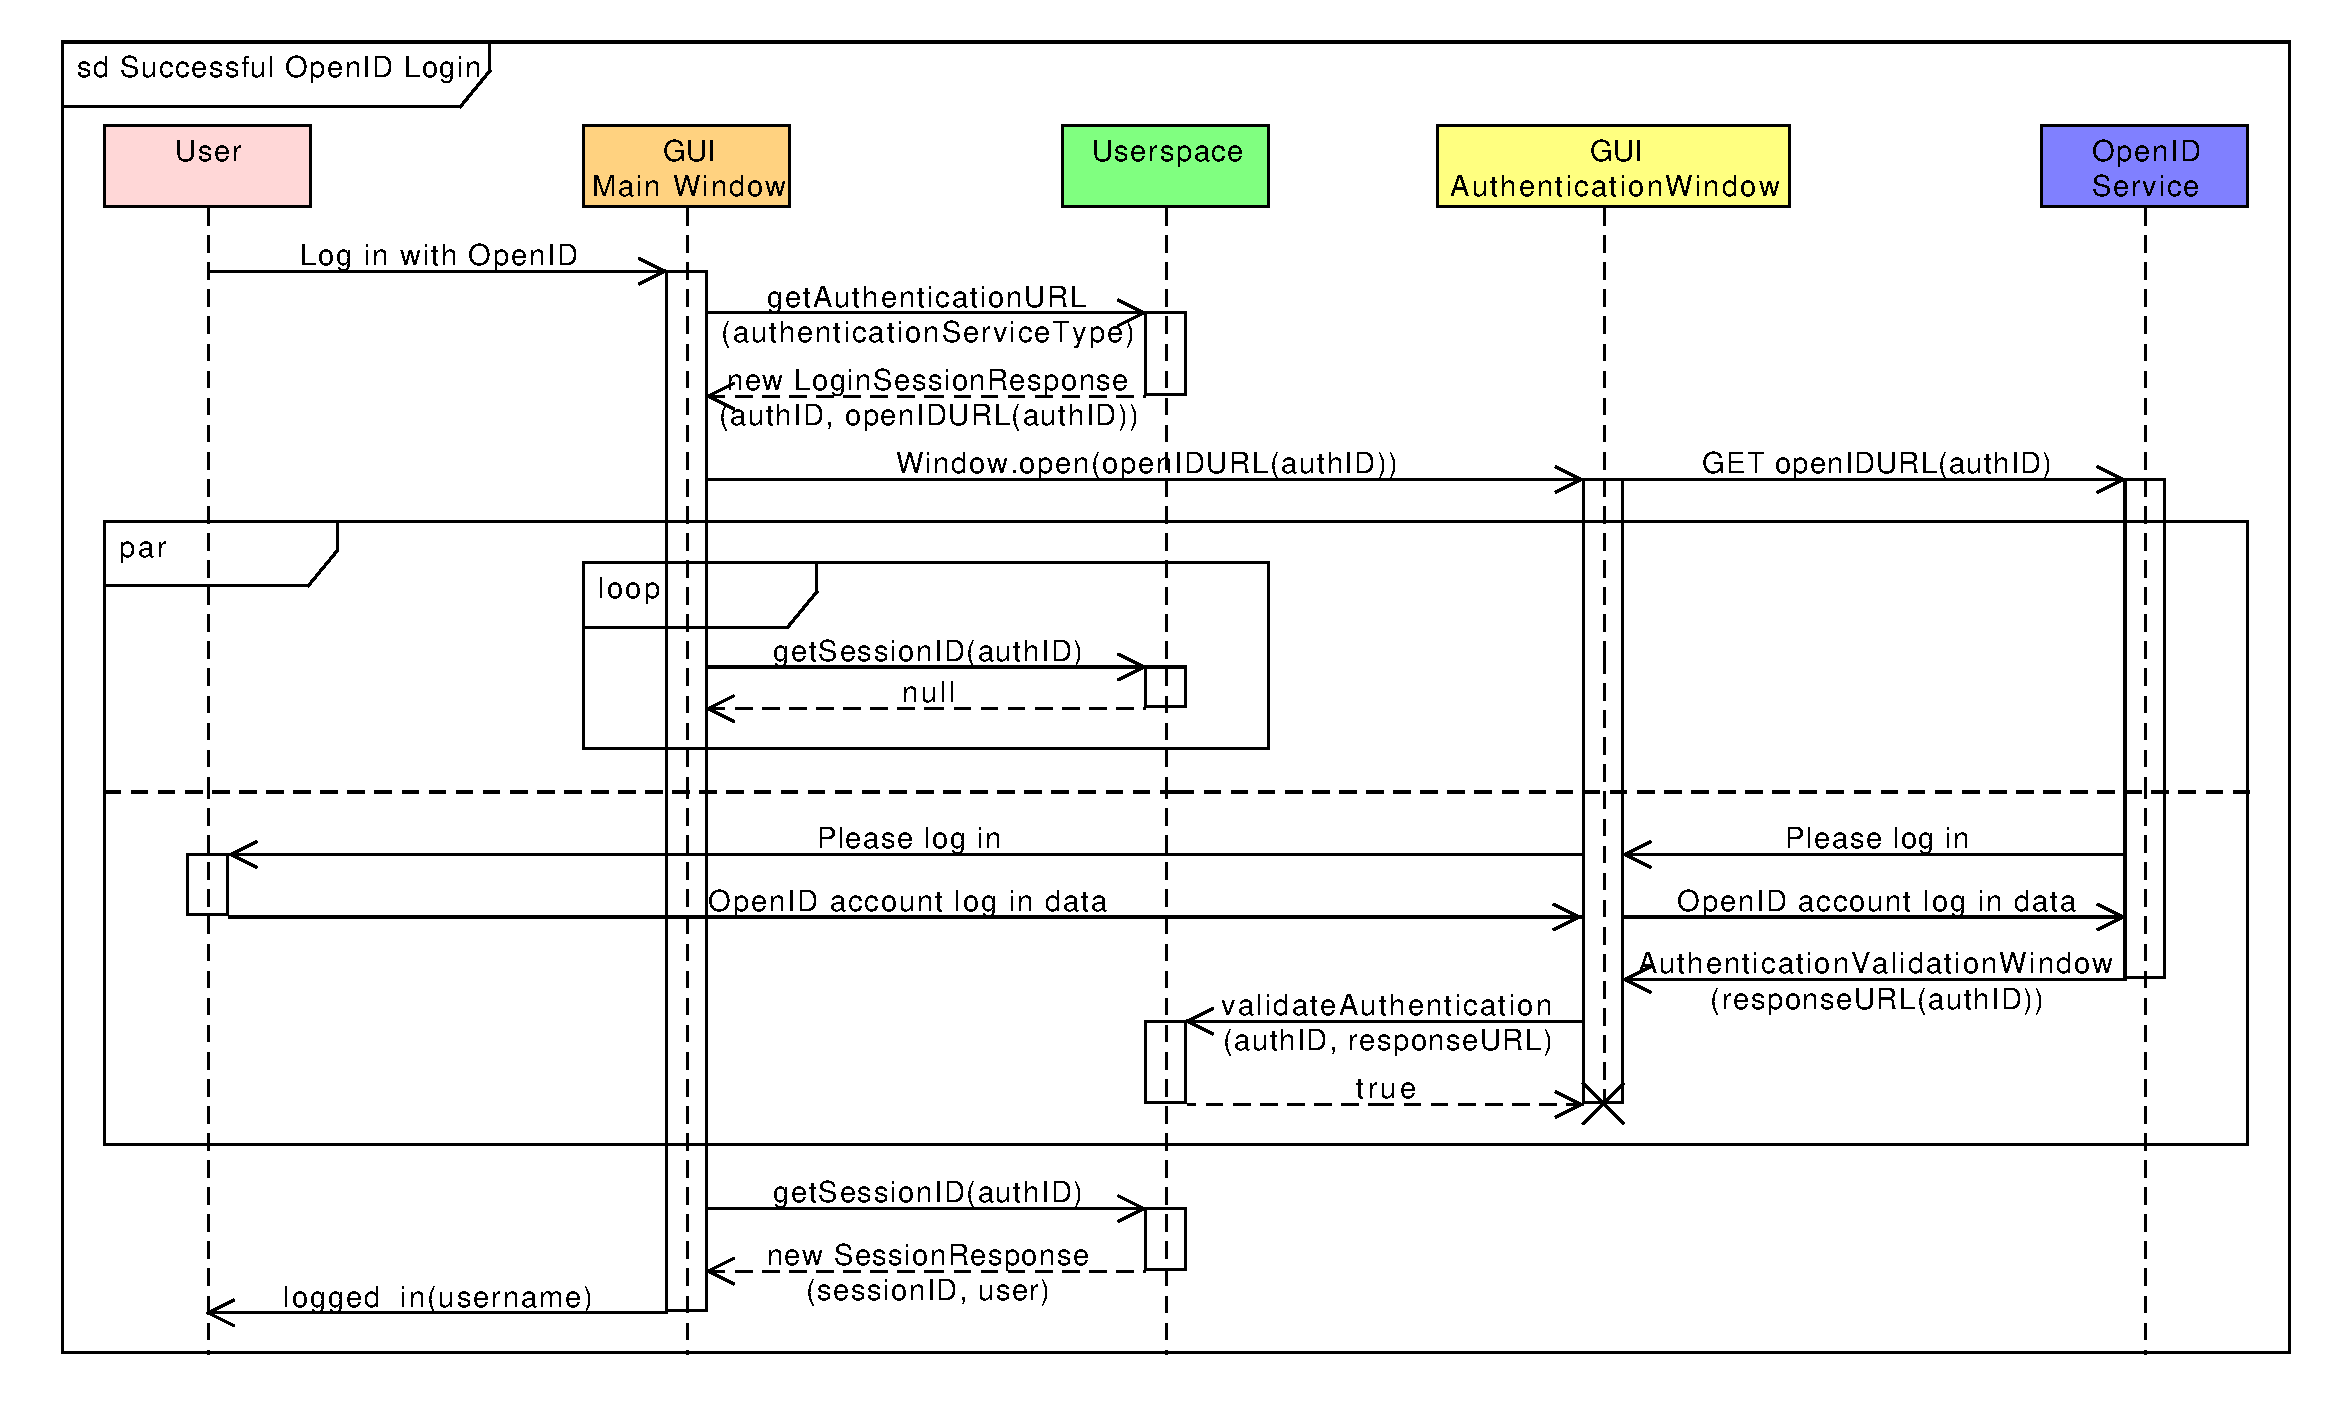
\includegraphics[scale=0.55, angle=90]{figures/openid_login_sequence.pdf}
\end{center}
\caption{Sequence diagram of OpenID login.}\label{gui:sd:openid_login}
\end{figure}
